\markboth{Anexos}{Anexos}
\Needspace{.42\textheight}\section{Reproducibilidad y decisiones de la versión}\label{anexo:reproducibilidad}
La versión \texttt{correcciones\_2026\_09\_10} conserva el protocolo temporal de la versión multiventana anterior. Los tres notebooks se ejecutaron en procesos Python nuevos. Los CSV originales se preservan; el respaldo previo de código, notebooks y plantilla está identificado en el registro de entrega. La autorización de trabajo y las diferencias de A3.1 y A2.5 se documentan sin presumir ratificación institucional.

Se contrastaron los clics, los días activos y el CV entre días activos sobre toda la fuente, para las inscripciones elegibles de los cinco cortes. También se comprobaron los límites de fechas, los indicadores candidatos y las etiquetas, así como que añadir información futura no modificara los predictores del corte. La alternativa sin duplicados exactos conserva la población y el evento. Los intervalos utilizan 5\,000 remuestreos de personas; su estabilidad numérica se examina comparando las primeras 500 y 2\,000 repeticiones con la secuencia completa. Esta comprobación no demuestra una convergencia universal.

El archivo \texttt{README\_\allowbreak{}REVISION.md} documenta los comandos de generación, comprobación e integración. Los registros independientes y las huellas digitales de los archivos permiten identificar la ejecución documentada y sus productos. No se entrenaron clasificadores ni se eligió una ventana óptima. La revisión bibliográfica del marco continúa parcial y el protocolo de validación predictiva permanece pendiente.

\subsection{Archivos de consulta de la revisión de datos}\label{kami:archivos}
La ejecución de los notebooks se documentó el 10 de septiembre de 2026. La edición de claridad del 30 de septiembre conserva esas salidas; no representa una nueva ejecución completa. La Tabla~\ref{kami:salidas} identifica las principales comprobaciones. Los nombres corresponden a archivos CSV del directorio de tablas de esa revisión.
\begingroup\small\setlength{\tabcolsep}{4pt}\renewcommand{\arraystretch}{1.16}
\begin{longtable}{p{.43\linewidth}p{.49\linewidth}}
\caption{Salidas que respaldan la revisión de datos.}\label{kami:salidas}\\
\toprule Archivo & Información que permite consultar \\\midrule\endfirsthead
\toprule Archivo & Información que permite consultar \\\midrule\endhead
\bottomrule\endfoot
\textnormal{01\_faltantes.csv} & Cantidad de campos vacíos y total de filas utilizado para cada porcentaje.\\
\textnormal{01\_rangos.csv} & Comprobaciones de calificaciones, clics y campos con valores restringidos.\\
\textnormal{01\_pesos.csv} & Cantidad de evaluaciones y suma de sus pesos por módulo, edición y grupo de evaluación.\\
\textnormal{01\_consistencia\_temporal.csv} & Fechas de matrícula, entrega y retiro que requieren una revisión específica.\\
\textnormal{02\_flujos.csv} & Cantidades que permanecen o se excluyen al aplicar cada condición por corte.\\
\textnormal{03\_efectos.csv} & Asociaciones entre indicadores y retiro futuro, junto con sus intervalos.\\
\end{longtable}\endgroup
El peso de una evaluación es su porcentaje asignado en el esquema de evaluación. Como ejemplo de la salida guardada, AAA en 2013J tiene cinco actividades de evaluación continua cuyos pesos suman 100 y un examen con peso 100. CCC en 2014B tiene ocho actividades que suman 100 y dos registros de examen que suman 200. Esta diferencia muestra por qué no se exigió una suma conjunta de 200 para todos los cursos; no demuestra por sí sola que exista un error en la fuente.

\Needspace{.42\textheight}\section{Resultados por nivel de las variables de contexto}\label{corr:anexocontexto}
Cada celda presenta el número de retiros futuros, el total de inscripciones elegibles de esa categoría y el porcentaje obtenido al dividir ambos conteos. Las columnas corresponden a días de corte; sus poblaciones y periodos de seguimiento pueden variar. Las categorías no disponibles permanecen explícitas y el análisis no atribuye causalidad ni certifica equidad.
\Needspace{0.2\textheight}
\begingroup\small\setlength{\tabcolsep}{3pt}\renewcommand{\arraystretch}{1.16}
\begin{longtable}{>{\raggedright\arraybackslash}p{0.225\linewidth}>{\raggedright\arraybackslash}p{0.135\linewidth}>{\raggedright\arraybackslash}p{0.135\linewidth}>{\raggedright\arraybackslash}p{0.135\linewidth}>{\raggedright\arraybackslash}p{0.135\linewidth}>{\raggedright\arraybackslash}p{0.135\linewidth}}
\caption{Retiros futuros / inscripciones elegibles (porcentaje) por nivel y corte.}\label{corr:niveles}\\
\toprule
\textbf{Nivel} & \textbf{7} & \textbf{14} & \textbf{28} & \textbf{42} & \textbf{56} \\
\midrule\endfirsthead
\toprule
\textbf{Nivel} & \textbf{7} & \textbf{14} & \textbf{28} & \textbf{42} & \textbf{56} \\
\midrule\endhead
\bottomrule\endfoot
Edad / 0-35 & 4\,796/20\,383 (23,5\%) & 3\,973/19\,575 (20,3\%) & 3\,550/19\,166 (18,5\%) & 3\,184/18\,800 (16,9\%) & 2\,825/18\,443 (15,3\%) \\
Edad / 35-55 & 1\,796/8\,491 (21,2\%) & 1\,571/8\,281 (19,0\%) & 1\,431/8\,156 (17,5\%) & 1\,288/8\,015 (16,1\%) & 1\,150/7\,878 (14,6\%) \\
Edad / 55<= & 40/202 (19,8\%) & 36/198 (18,2\%) & 31/193 (16,1\%) & 28/190 (14,7\%) & 23/185 (12,4\%) \\
Discapacidad / N & 5\,780/26\,298 (22,0\%) & 4\,833/25\,379 (19,0\%) & 4\,335/24\,908 (17,4\%) & 3\,886/24\,461 (15,9\%) & 3\,447/24\,025 (14,3\%) \\
Discapacidad / Y & 852/2\,778 (30,7\%) & 747/2\,675 (27,9\%) & 677/2\,607 (26,0\%) & 614/2\,544 (24,1\%) & 551/2\,481 (22,2\%) \\
IMD / 0-10\% & 773/2\,855 (27,1\%) & 622/2\,706 (23,0\%) & 560/2\,646 (21,2\%) & 514/2\,601 (19,8\%) & 458/2\,545 (18,0\%) \\
IMD / 10-20 & 765/3\,042 (25,1\%) & 610/2\,890 (21,1\%) & 541/2\,823 (19,2\%) & 495/2\,777 (17,8\%) & 443/2\,725 (16,3\%) \\
IMD / 20-30\% & 881/3\,217 (27,4\%) & 723/3\,060 (23,6\%) & 640/2\,979 (21,5\%) & 581/2\,920 (19,9\%) & 522/2\,861 (18,2\%) \\
IMD / 30-40\% & 733/3\,177 (23,1\%) & 604/3\,055 (19,8\%) & 541/2\,997 (18,1\%) & 483/2\,939 (16,4\%) & 425/2\,882 (14,7\%) \\
IMD / 40-50\% & 671/2\,886 (23,3\%) & 554/2\,773 (20,0\%) & 493/2\,714 (18,2\%) & 432/2\,653 (16,3\%) & 389/2\,611 (14,9\%) \\
IMD / 50-60\% & 590/2\,810 (21,0\%) & 515/2\,739 (18,8\%) & 462/2\,688 (17,2\%) & 409/2\,635 (15,5\%) & 362/2\,588 (14,0\%) \\
IMD / 60-70\% & 598/2\,640 (22,7\%) & 513/2\,559 (20,0\%) & 458/2\,509 (18,3\%) & 416/2\,467 (16,9\%) & 366/2\,417 (15,1\%) \\
IMD / 70-80\% & 526/2\,608 (20,2\%) & 464/2\,549 (18,2\%) & 426/2\,515 (16,9\%) & 378/2\,468 (15,3\%) & 328/2\,418 (13,6\%) \\
IMD / 80-90\% & 495/2\,485 (19,9\%) & 428/2\,418 (17,7\%) & 385/2\,377 (16,2\%) & 340/2\,332 (14,6\%) & 304/2\,297 (13,2\%) \\
IMD / 90-100\% & 428/2\,312 (18,5\%) & 383/2\,268 (16,9\%) & 354/2\,240 (15,8\%) & 314/2\,200 (14,3\%) & 279/2\,165 (12,9\%) \\
IMD / No disponible & 172/1\,044 (16,5\%) & 164/1\,037 (15,8\%) & 152/1\,027 (14,8\%) & 138/1\,013 (13,6\%) & 122/997 (12,2\%) \\
Región / East Anglian Region & 633/2\,962 (21,4\%) & 521/2\,851 (18,3\%) & 469/2\,803 (16,7\%) & 418/2\,752 (15,2\%) & 370/2\,707 (13,7\%) \\
Región / East Midlands Region & 510/2\,059 (24,8\%) & 416/1\,966 (21,2\%) & 372/1\,922 (19,4\%) & 339/1\,889 (17,9\%) & 299/1\,849 (16,2\%) \\
Región / Ireland & 221/1\,111 (19,9\%) & 214/1\,114 (19,2\%) & 192/1\,105 (17,4\%) & 172/1\,085 (15,9\%) & 156/1\,069 (14,6\%) \\
Región / London Region & 705/2\,815 (25,0\%) & 523/2\,635 (19,8\%) & 460/2\,572 (17,9\%) & 420/2\,532 (16,6\%) & 381/2\,493 (15,3\%) \\
Región / North Region & 386/1\,629 (23,7\%) & 322/1\,567 (20,5\%) & 283/1\,530 (18,5\%) & 262/1\,509 (17,4\%) & 231/1\,478 (15,6\%) \\
Región / North Western Region & 606/2\,479 (24,4\%) & 513/2\,390 (21,5\%) & 452/2\,331 (19,4\%) & 398/2\,277 (17,5\%) & 340/2\,219 (15,3\%) \\
Región / Scotland & 655/3\,202 (20,5\%) & 644/3\,192 (20,2\%) & 610/3\,160 (19,3\%) & 558/3\,108 (18,0\%) & 509/3\,059 (16,6\%) \\
Región / South East Region & 410/1\,872 (21,9\%) & 337/1\,799 (18,7\%) & 303/1\,767 (17,1\%) & 264/1\,729 (15,3\%) & 234/1\,699 (13,8\%) \\
Región / South Region & 586/2\,758 (21,2\%) & 501/2\,674 (18,7\%) & 447/2\,622 (17,0\%) & 401/2\,576 (15,6\%) & 350/2\,525 (13,9\%) \\
Región / South West Region & 512/2\,193 (23,3\%) & 411/2\,093 (19,6\%) & 369/2\,051 (18,0\%) & 335/2\,017 (16,6\%) & 310/1\,992 (15,6\%) \\
Región / Wales & 418/1\,983 (21,1\%) & 378/1\,944 (19,4\%) & 343/1\,910 (18,0\%) & 310/1\,877 (16,5\%) & 275/1\,842 (14,9\%) \\
Región / West Midlands Region & 568/2\,238 (25,4\%) & 459/2\,133 (21,5\%) & 413/2\,088 (19,8\%) & 362/2\,037 (17,8\%) & 325/2\,000 (16,2\%) \\
Región / Yorkshire Region & 422/1\,775 (23,8\%) & 341/1\,696 (20,1\%) & 299/1\,654 (18,1\%) & 261/1\,617 (16,1\%) & 218/1\,574 (13,9\%) \\
\end{longtable}\endgroup

\Needspace{.42\textheight}\section{Diccionario reconciliado de indicadores}\label{corr:anexodiccionario}
El diccionario permite relacionar los indicadores del texto con los nombres utilizados en el código. Se documentan 26 candidatos, incluidos ambos CV; no se han seleccionado variables mediante desempeño predictivo. El conteo de filas aparece únicamente como auditoría. Los identificadores, las variables de contexto y los desenlaces permanecen separados. En la tabla, $t$ es el día de corte; los intervalos de días incluyen ambos extremos. NaN identifica un valor que no puede calcularse con la información disponible, no un cero; SD significa desviación estándar. La función \texttt{floor} toma la parte entera inferior y permite contar semanas completas.
\Needspace{0.2\textheight}
\begingroup\small\setlength{\tabcolsep}{3pt}\renewcommand{\arraystretch}{1.16}
\begin{longtable}{>{\raggedright\arraybackslash}p{0.29\linewidth}>{\raggedright\arraybackslash}p{0.43\linewidth}>{\raggedright\arraybackslash}p{0.22\linewidth}}
\caption{Diccionario de candidatos y conteo de filas de auditoría; nombres idénticos al código.}\label{corr:diccionario}\\
\toprule
\textbf{Variable} & \textbf{Definición} & \textbf{Dominio y ausencia} \\
\midrule\endfirsthead
\toprule
\textbf{Variable} & \textbf{Definición} & \textbf{Dominio y ausencia} \\
\midrule\endhead
\bottomrule\endfoot
total\_\allowbreak{}clics & Suma de clics en 0..t & entero >= 0 \\
dias\_\allowbreak{}activos & Días con clics en 0..t & 0..t+1 \\
proporcion\_\allowbreak{}dias\_\allowbreak{}activos & dias\_\allowbreak{}activos/(t+1); calendario completo, no exposición individual & [0,1] \\
n\_\allowbreak{}registros\_\allowbreak{}vle & Filas de la fuente en 0..t; no son sesiones & entero >= 0 \\
promedio\_\allowbreak{}clics\_\allowbreak{}por\_\allowbreak{}dia\_\allowbreak{}activo & total\_\allowbreak{}clics/dias\_\allowbreak{}activos & NaN sin actividad \\
coef\_\allowbreak{}variacion\_\allowbreak{}clics & SD muestral de t+1 totales diarios / media; incluye ceros & NaN sin actividad \\
cv\_\allowbreak{}intensidad\_\allowbreak{}activa & SD muestral / media de clics solo en días activos; intensidad condicional & NaN si días activos < 2 \\
dias\_\allowbreak{}desde\_\allowbreak{}ultima\_\allowbreak{}interaccion & t - último día activo dentro de 0..t & NaN sin actividad \\
recencia\_\allowbreak{}relativa & Recencia/(t+1) & NaN sin actividad \\
semanas\_\allowbreak{}completas\_\allowbreak{}activas & Bloques completos de 7 días desde 0 con actividad; omite bloque final parcial & 0..floor((t+1)/7) \\
proporcion\_\allowbreak{}semanas\_\allowbreak{}completas\_\allowbreak{}activas & Semanas completas activas / floor((t+1)/7) & [0,1] \\
clics\_\allowbreak{}pre\_\allowbreak{}inicio & Clics con fecha < 0 & entero >= 0 \\
sin\_\allowbreak{}actividad\_\allowbreak{}acumulada & 1 si total\_\allowbreak{}clics=0 & 0/1 \\
sin\_\allowbreak{}actividad\_\allowbreak{}ultimos\_\allowbreak{}7d & 1 si no hay clics en t-6..t & NaN con menos de 7 días observados \\
sin\_\allowbreak{}actividad\_\allowbreak{}ultimos\_\allowbreak{}14d & 1 si no hay clics en t-13..t & NaN con menos de 14 días observados \\
sin\_\allowbreak{}actividad\_\allowbreak{}ultimos\_\allowbreak{}28d & 1 si no hay clics en t-27..t & NaN con menos de 28 días observados \\
clics\_\allowbreak{}ultimos\_\allowbreak{}7d & Clics en t-6..t & NaN si observación < 7 días \\
clics\_\allowbreak{}7d\_\allowbreak{}previos & Clics en t-13..t-7 & NaN si observación < 14 días \\
log\_\allowbreak{}ratio\_\allowbreak{}7d & ln((clics últimos 7d+1)/(clics 7d previos+1)) & NaN con historia <14 días o cero en ambos bloques \\
log\_\allowbreak{}ratio\_\allowbreak{}14d & Razón logarítmica suavizada entre últimos dos bloques de 14 días & NaN con historia <28 días o cero en ambos bloques \\
n\_\allowbreak{}evaluaciones\_\allowbreak{}entregadas & Evaluaciones no Exam ni banked entregadas en 0..t & entero >= 0 \\
n\_\allowbreak{}entregas\_\allowbreak{}pre\_\allowbreak{}inicio & Entregas no Exam ni banked anteriores a 0 & entero >= 0 \\
n\_\allowbreak{}evaluaciones\_\allowbreak{}programadas & Evaluaciones no Exam con fecha de calendario en 0..t & entero >= 0 \\
n\_\allowbreak{}programadas\_\allowbreak{}entregadas\_\allowbreak{}al\_\allowbreak{}corte & Evaluaciones programadas en 0..t entregadas hasta t, sin banked & 0..n programadas \\
proporcion\_\allowbreak{}programadas\_\allowbreak{}entregadas & Entregadas programadas / programadas; no mide puntualidad & NaN si no hay programadas \\
sin\_\allowbreak{}evaluacion\_\allowbreak{}programada & 1 si no existen evaluaciones programadas en 0..t & 0/1 \\
sin\_\allowbreak{}entregas\_\allowbreak{}acumuladas & 1 si no hay entregas no Exam ni banked en 0..t; no implica incumplimiento & 0/1 \\
\end{longtable}\endgroup

\Needspace{.42\textheight}\section{Enlace con la versión anterior y productos}
La versión anterior del corte 28 observaba actividad hasta el día 27. La versión actual incorpora también el día 28 y mantiene las 27\,515 inscripciones elegibles. Esta modificación explica cambios de cifras sin atribuirlos a alteraciones de las fuentes.

\Needspace{0.3\textheight}
\begingroup\small\setlength{\tabcolsep}{3pt}\renewcommand{\arraystretch}{1.16}
\begin{longtable}{>{\raggedright\arraybackslash}p{0.23\linewidth}>{\raggedright\arraybackslash}p{0.23\linewidth}>{\raggedright\arraybackslash}p{0.23\linewidth}>{\raggedright\arraybackslash}p{0.25\linewidth}}
\caption{Efecto de incluir el día 28 en las mismas inscripciones.}\label{multi02:enlace}\\
\toprule
\textbf{Indicador} & \textbf{Anterior} & \textbf{Actual} & \textbf{Inscripciones con cambio} \\
\midrule\endfirsthead
\toprule
\textbf{Indicador} & \textbf{Anterior} & \textbf{Actual} & \textbf{Inscripciones con cambio} \\
\midrule\endhead
\bottomrule\endfoot
Clics & 7\,603\,586 & 7\,766\,285 & 7\,993 \\*
Entregas & 22\,870 & 23\,136 & 263 \\*
\end{longtable}\endgroup
Se exportan conjuntos separados de datos auditables, predictores y etiquetas para cada corte; las claves se conservan para vincularlos, sin convertir el identificador de estudiante en predictor. El diccionario documenta 26 indicadores candidatos y separa las variables de contexto. La tabla apilada tiene una fila por inscripción y corte, no por persona. La intersección de los cinco conjuntos contiene 26\,429 inscripciones y se utiliza únicamente para una sensibilidad retrospectiva.

Los productos permiten continuar con un protocolo predictivo común. El ajuste de imputación, escalado, selección y cualquier remuestreo deberá realizarse dentro del entrenamiento de cada partición \cite{revsklearnpitfalls}. Esta fase no entrenó clasificadores, no seleccionó una ventana óptima y no ofrece evidencia de desempeño fuera de muestra. Antes de modelar deberán fijarse la generalización buscada y la separación por personas o presentaciones; una persona presente en varios cortes no debe contaminar conjuntos de entrenamiento y evaluación.



\clearpage
\Needspace{.42\textheight}\section{Esquema relacional OULAD}
\begin{figure}[H]\centering
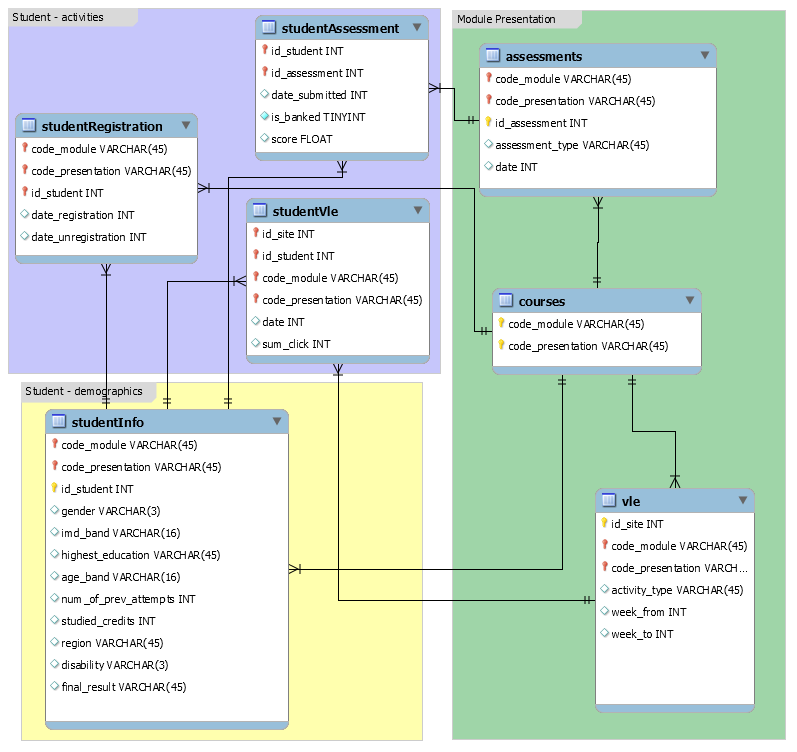
\includegraphics[width=.95\textwidth]{model.png}
\caption{Esquema relacional de OULAD. Fuente: \cite{sdata2017171}.}\label{fig:esquema-oulad}
\end{figure}

\clearpage
\section{Desarrollos matemáticos complementarios}\label{editorial:matematica}
Estas derivaciones explican la relación entre las formulaciones del marco teórico y sus condiciones matemáticas. Se conserva el detalle para consultar cómo se obtienen los resultados y bajo qué hipótesis son válidos. No constituyen evidencia de modelos entrenados.

\subsection{Varianza del promedio en Random Forest}\label{editorial:rf}
La proposición permite examinar por qué promediar árboles puede reducir la variación de las predicciones. Cada $T_b$ representa un estimador, $B$ cuenta los árboles, $\sigma_{\mathrm{RF}}^2$ es su varianza común y $\rho_{\mathrm{RF}}$ su correlación común por pares. Se trata de un caso idealizado que explicita las condiciones del resultado.
\begin{proposicion}[Varianza del promedio de estimadores correlacionados]\label{prop:rf-var}
Sean $B\geq2$ y $T_{1},\dots,T_{B}$ variables aleatorias con varianza común $\sigma_{\mathrm{RF}}^{2}>0$ y correlación común por pares $\rho_{\mathrm{RF}}$, con $-1/(B-1)\leq\rho_{\mathrm{RF}}\leq1$. Entonces
\begin{equation}\label{eq:rf-var}
\operatorname{Var}\!\left(\frac{1}{B}\sum_{b=1}^{B}T_{b}\right)
=\rho_{\mathrm{RF}}\,\sigma_{\mathrm{RF}}^{2}+\frac{1-\rho_{\mathrm{RF}}}{B}\,\sigma_{\mathrm{RF}}^{2}.
\end{equation}
\end{proposicion}
Bajo las hipótesis de la Proposición~\ref{prop:rf-var}, se obtiene la ecuación~\eqref{eq:rf-var} de la siguiente manera.
\begin{proof}
La expansión de la varianza da
\[
\frac{1}{B^2}\left[\sum_{b=1}^B\operatorname{Var}(T_b)+2\sum_{b<c}\operatorname{Cov}(T_b,T_c)\right]
=\frac{B\sigma_{\mathrm{RF}}^2+B(B-1)\rho_{\mathrm{RF}}\sigma_{\mathrm{RF}}^2}{B^2},
\]
que coincide con la ecuación~\eqref{eq:rf-var}. La condición sobre $\rho_{\mathrm{RF}}$ asegura que la matriz de correlación común sea semidefinida positiva.
\end{proof}
\subsection{Aproximación y solución por hojas en XGBoost}\label{editorial:xgb}
Se parte del objetivo de la ecuación~\eqref{eq:xgb-obj}, con $\nu=1$ para el árbol candidato. La expansión utiliza la puntuación acumulada de la etapa anterior.
Con $T$ como número de hojas y $\mathbf{w}$ como vector de pesos, se utiliza una expansión de Taylor de segundo orden de la pérdida en torno a la puntuación acumulada. Al omitir términos constantes respecto del árbol candidato, se obtiene:
\begin{equation}\label{eq:xgb-taylor}
\mathcal{L}^{(t_{\mathrm{boost}})}\simeq\sum_{i=1}^{n}\Big[g_{i}f_{t_{\mathrm{boost}}}(\mathbf{x}_{i})+\tfrac{1}{2}h_{i}f_{t_{\mathrm{boost}}}^{2}(\mathbf{x}_{i})\Big]+\Omega(f_{t_{\mathrm{boost}}}),
\qquad
g_{i}=\frac{\partial l}{\partial z_i^{(t_{\mathrm{boost}}-1)}},\;\;
h_{i}=\frac{\partial^{2}l}{\partial(z_i^{(t_{\mathrm{boost}}-1)})^{2}}.
\end{equation}
Para la pérdida logística esos términos adoptan la forma $g_{i}=\pi_{i}-y_{i}$ y $h_{i}=\pi_{i}(1-\pi_{i})$, con $\pi_{i}$ la probabilidad estimada en la iteración previa, lo que vincula el mecanismo del ensamble con la formulación de la ecuación \eqref{eq:logit} \cite{chen2016}.

Una vez fijadas las divisiones del árbol, se busca el peso que minimiza el objetivo de cada hoja. La siguiente proposición expresa ese peso mediante las sumas de derivadas y calcula cuánto mejora el objetivo al dividir una hoja en dos.

\begin{proposicion}[Peso óptimo de hoja y ganancia del corte]\label{prop:xgb}
Sea $I_{j}$ el conjunto de observaciones asignadas a la hoja $j$, $G_j=\sum_{i\in I_j}g_i$ y $H_j=\sum_{i\in I_j}h_i$. Se supone $\lambda_{\mathrm{XGB}}\geq0$, $\gamma_{\mathrm{XGB}}\geq0$ y $H_j+\lambda_{\mathrm{XGB}}>0$ en cada hoja. Fijada la estructura del árbol, el objetivo \eqref{eq:xgb-taylor} alcanza su mínimo en
\[
w_{j}^{\ast}=-\frac{\sum_{i\in I_{j}}g_{i}}{\sum_{i\in I_{j}}h_{i}+\lambda_{\mathrm{XGB}}},
\qquad
\tilde{\mathcal{L}}^{(t_{\mathrm{boost}})}=-\frac{1}{2}\sum_{j=1}^{T}\frac{\big(\sum_{i\in I_{j}}g_{i}\big)^{2}}{\sum_{i\in I_{j}}h_{i}+\lambda_{\mathrm{XGB}}}+\gamma_{\mathrm{XGB}} T,
\]
y la ganancia de un corte que divide $I$ en $I_{L}$ e $I_{R}$ es
\begin{equation}\label{eq:xgb-gain}
\mathcal{G}=\frac{1}{2}\left[
\frac{\big(\sum_{i\in I_{L}}g_{i}\big)^{2}}{\sum_{i\in I_{L}}h_{i}+\lambda_{\mathrm{XGB}}}
+\frac{\big(\sum_{i\in I_{R}}g_{i}\big)^{2}}{\sum_{i\in I_{R}}h_{i}+\lambda_{\mathrm{XGB}}}
-\frac{\big(\sum_{i\in I}g_{i}\big)^{2}}{\sum_{i\in I}h_{i}+\lambda_{\mathrm{XGB}}}
\right]-\gamma_{\mathrm{XGB}}.
\end{equation}
\end{proposicion}

Cada hoja aporta $G_jw_j+\tfrac12(H_j+\lambda_{\mathrm{XGB}})w_j^2$; su derivada se anula en el peso indicado y su segunda derivada es positiva bajo la hipótesis establecida. Al sustituir ese mínimo y comparar las dos hojas hijas con la hoja original se obtiene la ganancia de la ecuación~\eqref{eq:xgb-gain} \cite{chen2016}. 
\subsection{Condiciones de unicidad de la atribución SHAP}\label{editorial:shap}
Este resultado delimita cuándo las contribuciones de las variables quedan determinadas por las propiedades de la explicación. Una coalición es un conjunto de variables consideradas presentes; su función de valor establece la salida que se les asigna. La unicidad solo se afirma después de fijar esas elecciones.
\begin{teorema}[Unicidad de la atribución aditiva]\label{teo:shap}
Fijada la representación de presencia y ausencia de variables, la salida del modelo y la función de valor de las coaliciones, dentro de la clase de los modelos aditivos de atribución existe una única función que satisface simultáneamente exactitud local, ausencia de atribución a las variables no presentes y consistencia frente a cambios del modelo, y sus componentes son los valores de Shapley $\phi_{j}$.
\end{teorema}
El enunciado preciso y su demostración se remiten a \cite{lundberg2017,shapley1953}. El resultado presupone una función de valor, una representación y una salida fijadas; no establece igualdad entre explicaciones construidas con referencias distintas ni identifica relaciones causales. La lectura de las atribuciones conserva la escala de la ecuación~\eqref{eq:shap-aditivo}.

\subsection{Ajuste y regularización de la regresión logística}\label{clara:logistica}
El ajuste busca parámetros que asignen mayor probabilidad a las etiquetas observadas en el entrenamiento. La máxima verosimilitud lo expresa mediante la maximización de
\[
\ell(\beta_0,\boldsymbol{\beta})=\sum_{i=1}^{n}\Big[y_{i}\ln\pi_{i}+(1-y_{i})\ln(1-\pi_{i})\Big],
\qquad
\pi_{i}=\sigma_{\mathrm{log}}\big(\beta_0+\mathbf{x}_{i}^{\top}\boldsymbol{\beta}\big),
\]
Aquí $\ell$ es la log-verosimilitud, $y_i$ la etiqueta y $\pi_i$ la probabilidad estimada para la inscripción $i$; $n$ cuenta las inscripciones del entrenamiento. Cada término recompensa asignar una probabilidad alta a la clase observada. La solución no se obtiene mediante una fórmula cerrada: se aproxima actualizando los coeficientes de forma iterativa, habitualmente con Newton--Raphson expresado como mínimos cuadrados ponderados iterativamente \cite{hosmer2013,james2023}.

La interpretación de los coeficientes depende de la forma funcional y de las condiciones del ajuste. La ecuación \eqref{eq:logit} impone linealidad en la escala del \textit{logit}, por lo que el modelo no captura interacciones ni relaciones no monótonas, salvo que se especifiquen de forma explícita.

La inferencia convencional supone independencia entre observaciones, condición que requiere atención por las inscripciones repetidas. La estimación también puede resultar inestable ante colinealidad severa, condición frecuente entre variables de \textit{clickstream} que miden facetas próximas de la misma actividad. La separación completa de las clases por un predictor produce, en el límite, coeficientes divergentes y errores estándar inutilizables \cite{hosmer2013}. La regularización responde a los dos últimos problemas al penalizar la magnitud de los coeficientes:
\begin{equation}\label{eq:lr-reg}
(\hat\beta_0,\hat{\boldsymbol{\beta}})
=\arg\min_{\beta_0,\boldsymbol{\beta}}
\left\{-\ell(\beta_0,\boldsymbol{\beta})
+\lambda_{\mathrm{LR}}\Big[\tfrac{1}{2}(1-\alpha)\lVert\boldsymbol{\beta}\rVert_{2}^{2}
+\alpha\lVert\boldsymbol{\beta}\rVert_{1}\Big]\right\}.
\end{equation}
En la ecuación~\eqref{eq:lr-reg}, $\boldsymbol{\beta}$ reúne únicamente las pendientes: el intercepto $\beta_0$ se estima sin penalización. Se asume $\lambda_{\mathrm{LR}}\geq0$ y $0\leq\alpha\leq1$. El primero regula la intensidad de la penalización y el segundo combina la suma de cuadrados ($\ell_2$) con la suma de valores absolutos ($\ell_1$). Así, el objetivo equilibra el ajuste a las etiquetas y la magnitud de los coeficientes. La penalización $\ell_2$ contrae los coeficientes y la $\ell_1$ puede anular algunos de ellos; esto no garantiza que seleccione las variables verdaderamente relevantes. La relación entre $\lambda_{\mathrm{LR}}$ y un parámetro de implementación como $C$ depende también de si la pérdida se expresa como suma o promedio y de sus ponderaciones. La configuración deberá documentarse al entrenar. La regresión logística se conserva como modelo base interpretable, sin asumir de antemano que su desempeño igualará al de los ensambles.


\subsection{Procedimientos de eficiencia de LightGBM}\label{clara:lightgbm}
LightGBM utiliza histogramas para agrupar valores continuos y buscar cortes sobre un número reducido de intervalos. El coste de explorar un histograma con $k_{\mathrm{bins}}$ intervalos y $p$ variables es del orden de $O(k_{\mathrm{bins}}p)$; construirlo requiere recorrer las observaciones correspondientes. No se trata de un único coste $O(np)$ pagado para todo el entrenamiento: los histogramas se utilizan a lo largo de árboles y nodos, con optimizaciones como su obtención por diferencia \cite{revlightfeatures}.

El muestreo unilateral basado en gradientes (GOSS) busca reducir los casos utilizados sin perder la contribución de los que presentan mayores gradientes. El procedimiento conserva los $an$ casos de mayor magnitud de gradiente y selecciona otros $bn$ entre los restantes, con $0<a<1$ y $0<b\leq1-a$. Bajo la convención del algoritmo original, $b$ es una fracción del total $n$, no de los $(1-a)n$ restantes; el peso corrector es $(1-a)/b$ y el tamaño seleccionado es $(a+b)n$ \cite{ke2017}. Si se definiera $b$ como fracción de los restantes, esas dos expresiones cambiarían.

La agrupación de características excluyentes (EFB) combina variables que rara vez toman valores distintos de cero simultáneamente. Su propósito es reducir el trabajo sobre matrices dispersas, en las que predominan los ceros. Estas técnicas pueden mejorar la eficiencia, pero no garantizan igualdad de desempeño en todos los datos. Además, LightGBM suele expandir la hoja con mayor ganancia: profundidad y número de hojas deben controlarse conjuntamente. Un árbol binario de profundidad máxima $d_{\mathrm{arbol}}$ tiene a lo sumo $2^{d_{\mathrm{arbol}}}$ hojas. Elegir menos hojas puede ser una estrategia de regularización; la desigualdad estricta no es una condición matemática de comparación equitativa \cite{revlighttuning}.


\subsection{Máscaras y penalización de TabNet}\label{clara:tabnet}
TabNet es una arquitectura de aprendizaje profundo diseñada específicamente para datos tabulares, que procesa la entrada en $N_{s}$ pasos de decisión sucesivos. En cada paso $s_{\mathrm{TN}}$, un módulo de atención produce una máscara sobre las $p$ variables,
\[
\mathbf{M}[s_{\mathrm{TN}}]=\operatorname{sparsemax}\big(\mathbf{P}[s_{\mathrm{TN}}-1]\odot h_{s_{\mathrm{TN}}}(\mathbf{a}[s_{\mathrm{TN}}-1])\big),
\qquad
\mathbf{P}[s_{\mathrm{TN}}]=\prod_{j=1}^{s_{\mathrm{TN}}}\big(\gamma_{\mathrm{TN}}-\mathbf{M}[j]\big),
\]
En estas expresiones, $\mathbf a$ es el estado interno, $\mathbf M$ la máscara y $\mathbf P$ el factor que regula el uso previo de variables. El operador $\odot$ multiplica las componentes correspondientes y $\prod$ acumula esos factores entre pasos. La función $h_{s_{\mathrm{TN}}}$ es una transformación entrenable del estado del paso anterior y la función $\operatorname{sparsemax}$ normaliza la máscara de modo que sus componentes sumen uno y las de menor magnitud se anulen exactamente, a diferencia de la función \textit{softmax}. El término $\mathbf{P}[s_{\mathrm{TN}}]$ acumula el uso previo de cada variable y el parámetro $\gamma_{\mathrm{TN}}$ gobierna su reutilización: con $\gamma_{\mathrm{TN}}=1$ se reduce el prior de variables utilizadas, mientras valores mayores flexibilizan su reutilización. Como las máscaras son fraccionarias, la actualización del prior no establece por sí sola una exclusión binaria de toda variable previamente utilizada \cite{arXiv190807442}. 

Para favorecer máscaras que concentren el peso en pocas variables, se añade a la pérdida un término de entropía. La entropía mide cómo se reparte el peso entre las componentes de la máscara:
\[
L_{\text{disp}}=-\frac{1}{N_{s}N_{b}}\sum_{s_{\mathrm{TN}}=1}^{N_{s}}\sum_{b=1}^{N_{b}}\sum_{j=1}^{p}
\mathbf{M}_{b,j}[s_{\mathrm{TN}}]\,\log\big(\mathbf{M}_{b,j}[s_{\mathrm{TN}}]+\epsilon\big),
\]
Aquí $N_b$ es el número de casos del lote, $N_s$ el número de pasos y $\mathbf M_{b,j}[s_{\mathrm{TN}}]$ el peso de la variable $j$ para el caso $b$ en ese paso. El valor positivo $\epsilon$ estabiliza el logaritmo. El término se pondera con $\lambda_{\text{disp}}$; ese peso, el número de pasos y la dimensión de las representaciones internas son hiperparámetros que deberán ajustarse durante el entrenamiento.


\subsection{Cálculo de las contribuciones de Shapley}\label{clara:shapcalculo}
Dentro de las técnicas \textit{post-hoc}, SHAP (\textit{SHapley Additive exPlanations}) utiliza una formulación basada en la teoría de juegos. Su punto de partida es el valor de Shapley, solución de la teoría de juegos cooperativos que reparte el resultado conjunto de una coalición entre sus participantes según la contribución marginal promedio de cada uno sobre todos los órdenes posibles de incorporación \cite{shapley1953}. Trasladado a la predicción, el juego es la salida del modelo para una observación, los jugadores son las $p$ variables del conjunto $F$ y la atribución correspondiente a la variable $j$ resulta
\begin{equation}\label{eq:shapley}
\phi_{j}=\sum_{S\subseteq F\setminus\{j\}}
\frac{|S|!\,\big(p-|S|-1\big)!}{p!}
\Big[v\big(S\cup\{j\}\big)-v(S)\Big],
\end{equation}
Aquí $S$ recorre los subconjuntos de variables que no incluyen a $j$, y $v_x(S)$, abreviado como $v(S)$, es el valor asignado a cada conjunto para la observación $x$. La diferencia entre corchetes mide cuánto cambia ese valor al incorporar $j$. El símbolo $|S|$ cuenta sus variables y $!$ denota el factorial utilizado en la ponderación. Una elección condicional es $\mathbb{E}[f(X)\mid X_S=x_S]$: promedia la salida del modelo condicionada a los valores observados de las variables de $S$. Otra integra $f(x_S,X_{-S})$ sobre una distribución de referencia, fijando esas variables y variando las restantes. $X_S$ es el subvector de variables de $S$, $x_S$ sus valores observados y $X_{-S}$ las variables complementarias. Esas elecciones no son equivalentes en general y deben fijarse antes de calcular las atribuciones. El factor combinatorio pondera cada contribución marginal por la proporción de órdenes de incorporación en que se produce, de modo que la atribución no depende de un orden particular. La formulación unificada mostró que un conjunto de métodos de atribución previamente independientes, entre ellos las explicaciones locales por sustitución lineal, pertenecen a una misma clase de modelos aditivos de atribución, y estableció dentro de ella un resultado de unicidad.

